%!TEX root = /Users/velrok/Dropbox/TheoInf Seminar/Ausarbeitung/Main.tex

\section{Semantik} % (fold)
\label{sec:semantik}
Dieses Kapitel beschreibt die Semantik von Modal-Logik-Aussagen. 
Die Semantik wird dabei formal beschrieben. Die grundlegende Frage ist wann evaluiert eine Modal-Logik-Formel zu \emph{wahr} bzw. \emph{falsch}.\\
\\
Zur Erinnerung: In der \AL ist eine Interpretation eine mögliche Belegung der Variablen mit den Wahrheitswerten \emph{Wahr} oder \emph{Falsch}. Dabei muss jeder der Variablen einen dieser Werte annehmen.


Die Modal-Logik erfordert ein komplexeres Model für die Auswertung von Formeln, da verschiedene Arten von Wahr modelliert werden können \vglHuth{S. 308f}.
Ein Model in \ML wird deswegen durch eine \KS beschrieben. 

\begin{definition}
	\label{def:model}
	Ein Model $M$ einer \ML wird durch 3 Bestandteile beschrieben:
	\begin{itemize}
		\item Einer Menge von Welten $W$,
		\item einer Erreichbarkeitsfunktion $R$ auf $W$ ($R \subseteq W \times W$) und
		\item einer \fachwort{Labelingfunktion} $L : W \rightarrow P(Atome)$
	\end{itemize}
	%
	Man schreibt $R(x,y)$ um zu kennzeichnen, dass $(x,y)$ in $R$ enthalten ist. \citeHuth{S. 309}
\end{definition}


Nehmen wir an, die Menge der Welten $W$ sei
\begin{center}
	$\{ x_1, x_2, x_3, x_4, x_5, x_6 \}$
\end{center}
%
%
die Relation $R$ sei definiert als 
\begin{center}
	$\{(x_1, x_2), (x_1, x_3), (x_2, x_3), (x_3, x_2), (x_2, x_2), (x_4, x_5), (x_5, x_4), (x_5, x_6)\}$ 
\end{center}
%
%
und die Labelfunktion $L$ liefere
\begin{center}
	\begin{tabular}{c|cccccc}
		$x$ & $x_1$ & $x_2$ & $x_3$ & $x_4$ & $x_5$ & $x_6$\\
		\hline
		$L(x)$ & $\{q\}$ & $\{p,q\}$ & $\{p\}$ & $\{q\}$ & $\{\}$ & $\{p\}$
	\end{tabular}
\end{center}
%
%
dann ist Abbildung~\ref{fig:mmKripke01} die graphische Darstellung der beschriebenen \KS.

\begin{figure}[ht]
	\begin{center}
  	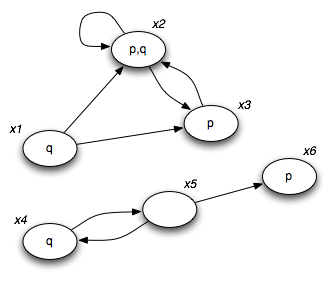
\includegraphics[width=0.65\textwidth]{./Images/Kripke01.png}
  	\caption{Beispiel einer Kripke-Struktur}
		\label{fig:mmKripke01}
	\end{center}
\end{figure}

\begin{definition}
	\label{def:reasoning}
	\label{eq:possibleWorlds}
	Sei $M = (W,R,L)$ ein Model einer \ML und $\phi$ sei eine Formel nach \eqref{eqn:bnf}.
	Dann lässt sich nach folgenden Regeln schließen ob $\phi$ in einer Welt $x$ \emph{Wahr} oder \emph{Falsch} ist.
	\begin{align}
	%	\begin{split}
		x &\Vdash \top\label{eqn:semanticTrue}\\
		x &\nVdash \bot\label{eqn:semanticFalse}\\
		x &\Vdash p\text{ gdw. }p \in L(x)\label{eqn:semanticLabel}\\
		x &\Vdash \neg \phi\text{ gdw. }x \nVdash \phi\\
		x &\Vdash \phi \wedge \psi\text{ gdw. }x \Vdash \phi\text{ und } x \Vdash \psi\label{eqn:semanticAnd}\\
		x &\Vdash \phi \vee \psi\text{ gdw. }x \Vdash \phi \text{, oder } x \Vdash \psi\\
		x &\Vdash \phi \rightarrow \psi\text{ gdw. }x \Vdash \psi\text{, immer wenn gilt }x \Vdash \phi\\
		x &\Vdash \phi \leftrightarrow \psi\text{ gdw. }( x \Vdash \phi\text{ gdw. }x \Vdash \psi)\label{eqn:semanticBiconditional}\\
		x &\Vdash \Box \psi \text{ gdw. }\forall y \in W \text{ gilt } R(x,y)\text{, und } y \Vdash \psi\label{eqn:semanticBox}\\
		x &\Vdash \Diamond \psi\text{ gdw. }\exists y \in W \text{ sodass }R(x,y)\text{ und }y \Vdash \psi\label{eqn:semanticDiamond}
	%	\end{split}
	\end{align}	
\end{definition}
\cite[S.310]{huth2004logic}\\
\\
%
%
Die Formeln \eqref{eqn:semanticTrue} und \eqref{eqn:semanticFalse} besagen, dass die Werte \true und \false enthalten sind. 

Die Formel \eqref{eqn:semanticLabel} besagt, dass wir Aussagen folgern können die Teil der Wissensbasis sind.

Die Formeln \eqref{eqn:semanticAnd} bis \eqref{eqn:semanticBiconditional} sind ähnlich zu denen aus der Aussagenlogik.

Besonders zu beachten sind die Formeln \eqref{eqn:semanticBox} und \eqref{eqn:semanticDiamond}. 
Die Formel \eqref{eqn:semanticBox} besagt, dass die Aussage $\Box\psi$ für eine Welt $x$ gefolgert werden kann, wenn $\psi$ in allen Welten $y$, die von $x$ aus erreichbar sind, folgerbar ist. 
Dies beinhaltet $x$ nur wenn $R(x,x)$ gilt.
Wichtig ist, dass die Aussage lediglich fordert, dass eine Aussage in allen \emph{erreichbaren} Welten gefolgert werden kann. 
$x \Vdash \Box \bot$ ist also \true wenn $x$ mit keiner anderen Welt verbunden ist.

Die Formel \eqref{eqn:semanticBox} ist ähnlich, nur das sie einen Existenz-Charakter hat. 
Aus $x$ lässt sich $\Diamond \psi$ folgern, wenn es mindestens eine Welt gibt, die von $x$ erreichbar ist, in der sich $\psi$ folgern lässt. 
Wichtig ist die Aussage, \emph{es existiert} eine Welt. 
$x \Vdash \Diamond \top$ ist also \false, wenn es keine Welt $x'$ gibt für die gilt: $R(x,x')$.\\


\begin{figure}[h!]
	\centering
	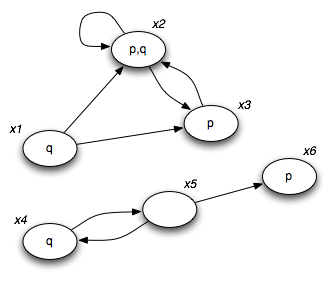
\includegraphics[height=6.5cm]{Images/Kripke01.png}
	\caption{Kripke Model Beispiel für Model Folgerungsbeispiele}
	\label{fig:Kripke01}
\end{figure}


\begin{definition}
	\label{def:model_erfuellt}
	Ein Model $\mathcal{M}$ einer \ML erfüllt eine Formel $\phi$, wenn jeder Zustand im Model die Formel erfüllt.
	Wir schreiben für diesen Fall $\mathcal{M} \vDash \psi$ gdw. $\forall x \in W, x \Vdash \psi$ gilt \citeHuth{S. 310f}.\\
\end{definition}
%
%
Anhand des \KMs in \Abb{Kripke01} werden nun ein paar Beispielformeln diskutiert, um die Definitionen zu veranschaulichen:

\begin{itemize}
	\item $x_1 \Vdash q$, gilt weil $q \in L(Lx_1)$
	\item $x_1 \Vdash \Diamond q$, weil es eine erreichbare Welt (hier $x_2$) $q \in L(x_2)$ gibt. Mathematisch formuliert: es gilt $R(x_1, x_2)$ und $x_2 \Vdash q$
	\item $x_1 \nVdash \Box q$, weil $R(x_1,x_3)$ und $x_3 \nVdash q$. $\Box$ setzt voraus, dass \emph{alle} erreichbaren Welten die Bedingung erfüllen.
	\item $x_5 \nVdash \Box p$ und $x_5 \nVdash \Box q$ sogar $x_5 \nVdash \Box p \vee \Box q$, allerdings gilt $x_5 \Vdash \Box (p \vee q)$. $x_5 \nVdash \Box p$ gilt, weil $x_4$ erreichbar ist, aber nicht $p$ enthält. $x_5 \nVdash \Box q$ gilt weil, $x_6$ erreichbar ist aber kein $q$ enthält. Damit gilt auch $x_5 \nVdash \Box p \vee \Box q$. $x_5 \Vdash \Box (p \vee q)$ gilt hingegen, weil alle erreichbaren Welten $(x_5, x_6)$ entweder $p$ oder $q$ enthalten.
	\item Die Welten die $\Box p \rightarrow p$ erfüllen sind: $x_2, x_3, x_4, x_5, x_6$.
	Die Welten $x_2, x_3, x_6$ erfüllen die Formeln mit \true, weil in ihnen $p$ enthalten ist und $\Box p$ gilt. Für $x_6$ gilt $\Box q$ weil es keine erreichbaren Welten hat (vgl. Formel \eqref{eqn:semanticBox} ).
	Die Welten $x_4, x_5$ erfüllen die Formel mit \false, weil sie $p$ nicht enthalten und nicht alle von ihnen erreichbaren Welten $p$ enthalten. $x_5 \nVdash \Box p$ ist der Fall, weil $x_4 \nVdash p$ zutrifft.
\end{itemize}
%
Welten wie $x_6$, die keine Verbindungen zu anderen Welten haben, erfordern besonderes Augenmerk.
Die Formel $x_6 \nVdash \Diamond \phi$ gilt z.B. immer, auch wenn $\phi = \top$ weil $\Diamond$ min eine verbundene Welt voraussetzt.
$x \nVdash \Diamond \top$ gilt z.B. immer wenn $x$ mindestens eine erreichbare Welt hat, weil $\top$ per Definition in jeder Welt erfüllt ist.
Ähnlich verhält es sich mit $x_6 \Vdash \Box \phi$. Diese Aussage gilt immer egal welchen Wert $\phi$ besitzt.
Das gilt auch für die Aussage $x_6 \Vdash \Box \bot$. 
Auch wenn $\bot$ per Definition in jeder Welt \false ist, ist die Aussage $x_6 \Vdash \Box \bot$ \true, wenn es keine anderen verbundenen Welten gibt.
Es ist schlichtweg nicht möglich das Gegenteil zu beweisen, weil es keine Gegenbeispiele geben kann.
Auch wenn diese Interpretationen nicht intuitiv sind, sichern sie die \deMorganBedingung, siehe \eqref{eqn:semanticBox}.
%
%
\paragraph{\formelSchemata} % (fold)
\label{par:formel_schemata}
\formelSchemata beschreiben eine generelle Form, ein Pattern von Formeln.
Jede Belegung eines solchen \formelSchematas wird \fachwort{Instanz} genannt.
Die Anzahl der möglichen Instanzen ist unendlich.\\
\\
Hier ein paar Instanzen-Beispiele für das \formelSchema $\psi \rightarrow \Box \Diamond \psi$:\\
\begin{itemize}
	\item $p \rightarrow \Box \Diamond p$
	\item $q \rightarrow \Box \Diamond q$
	\item $(p \wedge r \rightarrow q) \rightarrow \Box \Diamond (p \wedge r \rightarrow q)$
\end{itemize}
%
%
Es gilt eine Welt / ein Model erfüllt ein Formelschema, wenn es \emph{alle} seine \emph{Instanzen} erfüllt. 
Es reicht nicht aus wenn nur eine Instanz erfüllt wird. 
Bsp.: Wenn alle Welten eines Models die Formel $\neg p \wedge q$, aber nur eine die Formel $\neg q \wedge p$ nicht erfüllt, dann ist das Schema $\neg \phi \wedge \psi$ \emph{nicht} erfüllt.
% paragraph formel_schemata (end)


\paragraph{Äquvivalenz zwischen modal logischen Formeln} % (fold)
\label{par:gleichheit}
%
\begin{definition}
	\label{def:model_folgert}
	\begin{itemize}
		\item Eine Menge von modal logischen Formeln $\Gamma$ folgert eine modal logische Formel $\psi$, gdw. wenn für jede Welt $w$ aus jedem Model $\mathcal{M}$ gilt $x \Vdash \psi$ immer wenn gilt $x \Vdash \phi$ $\forall \phi \in \Gamma$. 
		Dies wird notiert durch $\Gamma \vDash \psi$.
		\item Wir bezeichnen zwei modal logische Formeln $\phi$ und $\psi$ als semantisch äquivalente wenn sowohl $\psi \vDash \phi$ als auch $\psi \vDash \phi$ gilt und notieren dies mit $\psi \equiv \phi$.\\
		\cite[S.313]{huth2004logic}
	\end{itemize}	
\end{definition}
%
$\phi \equiv \psi$ gilt sobald \emph{eine} Welt in \emph{einem} Model sowohl die eine als auch die andere Formel erfüllt.
Alle Äquivalenzen aus der Aussagenlogik gelten auch für die \ML wenn man sie in dasselbe Schema überträgt.\\
Zudem gelten für $\Box$ und $\Diamond$ die \deMorganRegeln.\\
\begin{equation}
	\neg \Box \phi \equiv \Diamond \neg \phi \text{ und } \neg \Diamond \phi \equiv \Box \neg \phi
\end{equation}
%
Außerdem distributiert $\Box$ über $\wedge$ und $\Diamond$ über $\vee$, aber nicht umgekehrt. \cite[S.314]{huth2004logic}
\begin{equation}
	\Box(\phi \wedge \psi) \equiv \Box \phi \wedge \Box \psi \text{ und }
	\Diamond(\phi \vee \psi) \equiv \Diamond \phi \vee \Diamond \psi
\end{equation}


% paragraph paragraph_name (end)

\paragraph{Valide Formeln} % (fold)
\label{par:paragraph_name}

\begin{definition}
	\label{def:valide}
	Eine modal logische Formel $\psi$ wird valide genant wenn sie in jeder Welt in jedem Model \true ist, also gdw. $\vDash \psi$ gilt \citeHuth{S. 314}.
\end{definition}

%
Alle Tautologien sind valide Formeln.
Dies ist z.B.: bei $\neg \Box \phi \leftrightarrow \Diamond \neg \psi$ der Fall.
(Beweis siehe \cite[S.314]{huth2004logic}).\\
Eine besonders wichtige Formel ist die K Formel: \KFormel .
Sie wird in der Literatur zu Ehren des Erfinders der Kripke-Strukturen und der hier behandelten \PW Semantik (siehe Formel-Block \eqref{eq:possibleWorlds}), S. Kripke mit $K$ abgekürzt.\\
\\
Um $K$ zu beweisen gehen wir davon aus, dass es ein Model \modelFormel mit einer Welt $x$ gibt und für $x$ $\Box(\phi \rightarrow \psi) \wedge \Box \phi$ gilt.\\
Um die Formel zu beweisen, müssen wir mit Hilfe der Regeln aus \eqref{eq:possibleWorlds} $x \Vdash \Box \psi$ nachweisen.\\
Dies ist der Fall:\\
gdw. $x \Vdash \Box(\phi \rightarrow \psi)$ und $x \Vdash \Box \phi$\\
gdw. $\forall y$ mit $R(x,y)$ gilt: $y \Vdash \phi \rightarrow \psi$ und $y \Vdash \phi$. Woraus $y \Vdash \psi$ folgt.\\
gdw. $x \Vdash \Box \psi$\\
\\
In der einfachen \ML $K$ gibt es keine weiteren interessanten validen Formeln.\cite[S.314]{huth2004logic}\\
\\
Dadurch das man bestimme Formeln als valide voraussetzt, kann man eigene Logiken und damit andere Modalitäten von \true erzeugen.
Die \NML $K$ schreibt nur die Validität von $K$ vor.\\
Im nächsten Kapitel werden weitere Formeln, die als valide vorausgesetzt werden können, vorgestellt und deren Auswirkungen diskutiert.


% paragraph paragraph_name (end)







% section semantik (end)
